\chapter{FOLDER STRUCTURE}

The Shopify application follows a specific directory layout enforced by the Laravel framework and the React/Inertia frontend integration. This structure separates concerns efficiently, placing routing, controllers, models, and frontend views in their designated areas.

\begin{figure}[H]
    \centering
    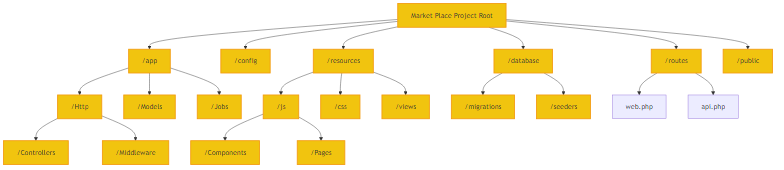
\includegraphics[width=0.8\textwidth]{folder_structure.png}
    \caption{Shopify Project Folder Structure}
    \label{fig:folder_structure}
\end{figure}

\section{Key Directories}
\begin{itemize}
    \item \textbf{\texttt{app/}}: Contains the core business logic of the application, including HTTP Controllers (\texttt{app/Http/Controllers}), Eloquent Models (\texttt{app/Models}), and Middleware.
    \item \textbf{\texttt{bootstrap/}}: Holds the file that bootstraps the Laravel framework and configures auto-loading.
    \item \textbf{\texttt{config/}}: Contains all of the base configuration files for the application such as database, authentication, and session settings.
    \item \textbf{\texttt{database/}}: Houses database migrations (\texttt{database/migrations}) to build tables, alongside model factories and data seeders.
    \item \textbf{\texttt{public/}}: The document root for the web server, containing the \texttt{index.php} entry point and compiled Vite static assets (\texttt{public/build}).
    \item \textbf{\texttt{resources/}}: Contains the raw, uncompiled assets such as the React components (inside \texttt{resources/js/Pages} and \texttt{resources/js/Components}), CSS files (like \texttt{app.css} using Tailwind), and localization files.
    \item \textbf{\texttt{routes/}}: Defines all route definitions for the application, specifically \texttt{web.php} which maps URLs to Controllers and renders Inertia views.
    \item \textbf{\texttt{storage/}}: Contains compiled Blade templates, file-based sessions, file caches, and other files generated automatically by the platform.
\end{itemize}
